% Options for packages loaded elsewhere
\PassOptionsToPackage{unicode}{hyperref}
\PassOptionsToPackage{hyphens}{url}
%
\documentclass[
]{article}
\usepackage{amsmath,amssymb}
\usepackage{iftex}
\ifPDFTeX
  \usepackage[T1]{fontenc}
  \usepackage[utf8]{inputenc}
  \usepackage{textcomp} % provide euro and other symbols
\else % if luatex or xetex
  \usepackage{unicode-math} % this also loads fontspec
  \defaultfontfeatures{Scale=MatchLowercase}
  \defaultfontfeatures[\rmfamily]{Ligatures=TeX,Scale=1}
\fi
\usepackage{lmodern}
\ifPDFTeX\else
  % xetex/luatex font selection
\fi
% Use upquote if available, for straight quotes in verbatim environments
\IfFileExists{upquote.sty}{\usepackage{upquote}}{}
\IfFileExists{microtype.sty}{% use microtype if available
  \usepackage[]{microtype}
  \UseMicrotypeSet[protrusion]{basicmath} % disable protrusion for tt fonts
}{}
\makeatletter
\@ifundefined{KOMAClassName}{% if non-KOMA class
  \IfFileExists{parskip.sty}{%
    \usepackage{parskip}
  }{% else
    \setlength{\parindent}{0pt}
    \setlength{\parskip}{6pt plus 2pt minus 1pt}}
}{% if KOMA class
  \KOMAoptions{parskip=half}}
\makeatother
\usepackage{xcolor}
\usepackage[margin=1in]{geometry}
\usepackage{color}
\usepackage{fancyvrb}
\newcommand{\VerbBar}{|}
\newcommand{\VERB}{\Verb[commandchars=\\\{\}]}
\DefineVerbatimEnvironment{Highlighting}{Verbatim}{commandchars=\\\{\}}
% Add ',fontsize=\small' for more characters per line
\usepackage{framed}
\definecolor{shadecolor}{RGB}{248,248,248}
\newenvironment{Shaded}{\begin{snugshade}}{\end{snugshade}}
\newcommand{\AlertTok}[1]{\textcolor[rgb]{0.94,0.16,0.16}{#1}}
\newcommand{\AnnotationTok}[1]{\textcolor[rgb]{0.56,0.35,0.01}{\textbf{\textit{#1}}}}
\newcommand{\AttributeTok}[1]{\textcolor[rgb]{0.13,0.29,0.53}{#1}}
\newcommand{\BaseNTok}[1]{\textcolor[rgb]{0.00,0.00,0.81}{#1}}
\newcommand{\BuiltInTok}[1]{#1}
\newcommand{\CharTok}[1]{\textcolor[rgb]{0.31,0.60,0.02}{#1}}
\newcommand{\CommentTok}[1]{\textcolor[rgb]{0.56,0.35,0.01}{\textit{#1}}}
\newcommand{\CommentVarTok}[1]{\textcolor[rgb]{0.56,0.35,0.01}{\textbf{\textit{#1}}}}
\newcommand{\ConstantTok}[1]{\textcolor[rgb]{0.56,0.35,0.01}{#1}}
\newcommand{\ControlFlowTok}[1]{\textcolor[rgb]{0.13,0.29,0.53}{\textbf{#1}}}
\newcommand{\DataTypeTok}[1]{\textcolor[rgb]{0.13,0.29,0.53}{#1}}
\newcommand{\DecValTok}[1]{\textcolor[rgb]{0.00,0.00,0.81}{#1}}
\newcommand{\DocumentationTok}[1]{\textcolor[rgb]{0.56,0.35,0.01}{\textbf{\textit{#1}}}}
\newcommand{\ErrorTok}[1]{\textcolor[rgb]{0.64,0.00,0.00}{\textbf{#1}}}
\newcommand{\ExtensionTok}[1]{#1}
\newcommand{\FloatTok}[1]{\textcolor[rgb]{0.00,0.00,0.81}{#1}}
\newcommand{\FunctionTok}[1]{\textcolor[rgb]{0.13,0.29,0.53}{\textbf{#1}}}
\newcommand{\ImportTok}[1]{#1}
\newcommand{\InformationTok}[1]{\textcolor[rgb]{0.56,0.35,0.01}{\textbf{\textit{#1}}}}
\newcommand{\KeywordTok}[1]{\textcolor[rgb]{0.13,0.29,0.53}{\textbf{#1}}}
\newcommand{\NormalTok}[1]{#1}
\newcommand{\OperatorTok}[1]{\textcolor[rgb]{0.81,0.36,0.00}{\textbf{#1}}}
\newcommand{\OtherTok}[1]{\textcolor[rgb]{0.56,0.35,0.01}{#1}}
\newcommand{\PreprocessorTok}[1]{\textcolor[rgb]{0.56,0.35,0.01}{\textit{#1}}}
\newcommand{\RegionMarkerTok}[1]{#1}
\newcommand{\SpecialCharTok}[1]{\textcolor[rgb]{0.81,0.36,0.00}{\textbf{#1}}}
\newcommand{\SpecialStringTok}[1]{\textcolor[rgb]{0.31,0.60,0.02}{#1}}
\newcommand{\StringTok}[1]{\textcolor[rgb]{0.31,0.60,0.02}{#1}}
\newcommand{\VariableTok}[1]{\textcolor[rgb]{0.00,0.00,0.00}{#1}}
\newcommand{\VerbatimStringTok}[1]{\textcolor[rgb]{0.31,0.60,0.02}{#1}}
\newcommand{\WarningTok}[1]{\textcolor[rgb]{0.56,0.35,0.01}{\textbf{\textit{#1}}}}
\usepackage{graphicx}
\makeatletter
\def\maxwidth{\ifdim\Gin@nat@width>\linewidth\linewidth\else\Gin@nat@width\fi}
\def\maxheight{\ifdim\Gin@nat@height>\textheight\textheight\else\Gin@nat@height\fi}
\makeatother
% Scale images if necessary, so that they will not overflow the page
% margins by default, and it is still possible to overwrite the defaults
% using explicit options in \includegraphics[width, height, ...]{}
\setkeys{Gin}{width=\maxwidth,height=\maxheight,keepaspectratio}
% Set default figure placement to htbp
\makeatletter
\def\fps@figure{htbp}
\makeatother
\setlength{\emergencystretch}{3em} % prevent overfull lines
\providecommand{\tightlist}{%
  \setlength{\itemsep}{0pt}\setlength{\parskip}{0pt}}
\setcounter{secnumdepth}{5}
\usepackage{float} \floatplacement{figure}{H} \usepackage{caption} \captionsetup[figure]{font=scriptsize}
\usepackage{booktabs}
\usepackage{longtable}
\usepackage{array}
\usepackage{multirow}
\usepackage{wrapfig}
\usepackage{float}
\usepackage{colortbl}
\usepackage{pdflscape}
\usepackage{tabu}
\usepackage{threeparttable}
\usepackage{threeparttablex}
\usepackage[normalem]{ulem}
\usepackage{makecell}
\usepackage{xcolor}
\ifLuaTeX
  \usepackage{selnolig}  % disable illegal ligatures
\fi
\IfFileExists{bookmark.sty}{\usepackage{bookmark}}{\usepackage{hyperref}}
\IfFileExists{xurl.sty}{\usepackage{xurl}}{} % add URL line breaks if available
\urlstyle{same}
\hypersetup{
  pdftitle={STA2005S - Regression Assignment},
  hidelinks,
  pdfcreator={LaTeX via pandoc}}

\title{STA2005S - Regression Assignment}
\author{true \and true}
\date{2024-10-16}

\begin{document}
\maketitle

\newpage

\hypertarget{part-one-analysis}{%
\subsection{Part One : Analysis}\label{part-one-analysis}}

\hypertarget{section-1-introduction}{%
\section{Section 1: Introduction}\label{section-1-introduction}}

Air pollution, particularly high levels of particulate matter (PM), is a
major environmental and public health issue in South Africa's urban
centers. Exposure to elevated PM levels is linked to respiratory
diseases and other serious health conditions. Understanding the factors
influencing PM concentrations is crucial for developing policies that
improve air quality and protect public health. This analysis seeks to
identify the key drivers of air pollution in South Africa's cities,
focusing on how various urban, environmental, and socioeconomic factors
affect particulate matter levels.\\
Unknown Factors to Investigate:\\
Traffic Density: How do varying levels of vehicle traffic contribute to
PM levels in different areas?\\
Industrial Activity: What is the impact of industrial activity near
monitoring stations on air quality?\\
Temperature \& Humidity: How do changes in weather conditions, like
temperature and humidity, influence PM concentrations?\\
Wind Speed: How does wind speed affect the dispersion or accumulation of
particulate matter in urban areas?\\
Day of the Week \& Public Holidays: Do patterns of human activity on
weekdays, weekends, and holidays significantly influence pollution
levels?\\
Urban Greenery: How effective are green spaces in reducing air pollution
in densely populated areas?

\hypertarget{objective}{%
\section{Objective}\label{objective}}

\hfill\break
The goal of this analysis is to explore the relationships between PM
levels and these explanatory variables. By identifying the most
influential factors, we aim to inform urban planning and public health
strategies that address air pollution and improve the quality of life in
South African cities.

\hypertarget{section-2-data-exploration}{%
\subsection{Section 2 : Data
Exploration}\label{section-2-data-exploration}}

density plot

pairwsie plots

\begin{Shaded}
\begin{Highlighting}[]
\NormalTok{continuous\_vars }\OtherTok{\textless{}{-}}\NormalTok{ data\_tidy\_air\_quality[, }\FunctionTok{sapply}\NormalTok{(data\_tidy\_air\_quality, is.numeric)]}
\FunctionTok{pairs}\NormalTok{(continuous\_vars, }\AttributeTok{main =} \StringTok{"Pairwise Scatterplots of Continuous Variables"}\NormalTok{)}
\end{Highlighting}
\end{Shaded}

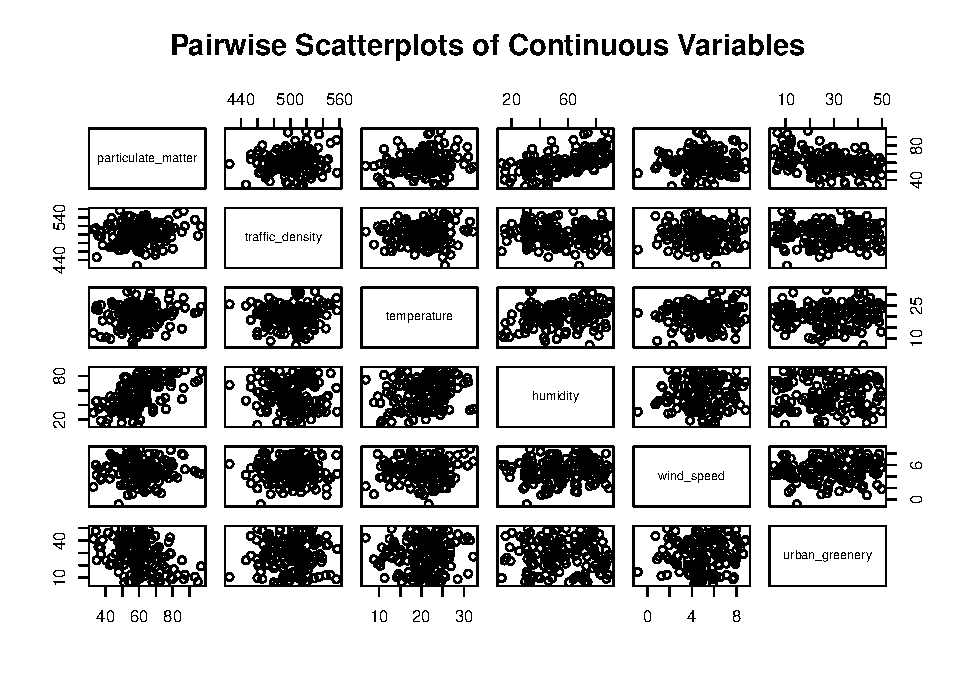
\includegraphics{Report_files/figure-latex/unnamed-chunk-1-1.pdf}

categorial variable plots

\begin{Shaded}
\begin{Highlighting}[]
\NormalTok{data\_tidy\_air\_quality}\SpecialCharTok{$}\NormalTok{industrial\_activity }\OtherTok{\textless{}{-}} \FunctionTok{factor}\NormalTok{(data\_tidy\_air\_quality}\SpecialCharTok{$}\NormalTok{industrial\_activity, }
                                   \AttributeTok{levels =} \FunctionTok{c}\NormalTok{(}\StringTok{"None"}\NormalTok{,}\StringTok{"Low"}\NormalTok{, }\StringTok{"Moderate"}\NormalTok{, }\StringTok{"High"}\NormalTok{))  }\CommentTok{\# Adjust the levels according to your data}

\NormalTok{data\_tidy\_air\_quality}\SpecialCharTok{$}\NormalTok{day\_of\_week }\OtherTok{\textless{}{-}} \FunctionTok{factor}\NormalTok{(data\_tidy\_air\_quality}\SpecialCharTok{$}\NormalTok{day\_of\_week, }
                           \AttributeTok{levels =} \FunctionTok{c}\NormalTok{(}\StringTok{"Monday"}\NormalTok{, }\StringTok{"Tuesday"}\NormalTok{, }\StringTok{"Wednesday"}\NormalTok{, }
                                      \StringTok{"Thursday"}\NormalTok{, }\StringTok{"Friday"}\NormalTok{, }\StringTok{"Saturday"}\NormalTok{, }\StringTok{"Sunday"}\NormalTok{))}

\NormalTok{data\_tidy\_air\_quality}\SpecialCharTok{$}\NormalTok{holiday }\OtherTok{\textless{}{-}} \FunctionTok{factor}\NormalTok{(data\_tidy\_air\_quality}\SpecialCharTok{$}\NormalTok{holiday, }
                           \AttributeTok{levels =} \FunctionTok{c}\NormalTok{(}\StringTok{"Yes"}\NormalTok{, }\StringTok{"No"}\NormalTok{))}

\NormalTok{categorical\_vars }\OtherTok{\textless{}{-}} \FunctionTok{names}\NormalTok{(data\_tidy\_air\_quality)[}\FunctionTok{sapply}\NormalTok{(data\_tidy\_air\_quality, is.factor)]}


\ControlFlowTok{for}\NormalTok{ (var }\ControlFlowTok{in}\NormalTok{ categorical\_vars) \{}
\NormalTok{  plt}\OtherTok{\textless{}{-}} \FunctionTok{ggplot}\NormalTok{(data\_tidy\_air\_quality, }\FunctionTok{aes\_string}\NormalTok{(}\AttributeTok{x =}\NormalTok{ var, }\AttributeTok{y =} \StringTok{"particulate\_matter"}\NormalTok{)) }\SpecialCharTok{+}
    \FunctionTok{geom\_boxplot}\NormalTok{() }\SpecialCharTok{+}
    \FunctionTok{labs}\NormalTok{(}\AttributeTok{title =} \FunctionTok{paste}\NormalTok{(}\StringTok{"Particulate Matter vs"}\NormalTok{, var),}
         \AttributeTok{x =}\NormalTok{ var,}
         \AttributeTok{y =} \StringTok{"Particulate Matter"}\NormalTok{) }\SpecialCharTok{+}
    \FunctionTok{theme\_minimal}\NormalTok{() }
    
  
  \FunctionTok{print}\NormalTok{(plt)  }\CommentTok{\# Print the plot}
\NormalTok{\}}
\end{Highlighting}
\end{Shaded}

\begin{verbatim}
## Warning: `aes_string()` was deprecated in ggplot2 3.0.0.
## i Please use tidy evaluation idioms with `aes()`.
## i See also `vignette("ggplot2-in-packages")` for more information.
## This warning is displayed once every 8 hours.
## Call `lifecycle::last_lifecycle_warnings()` to see where this warning was
## generated.
\end{verbatim}

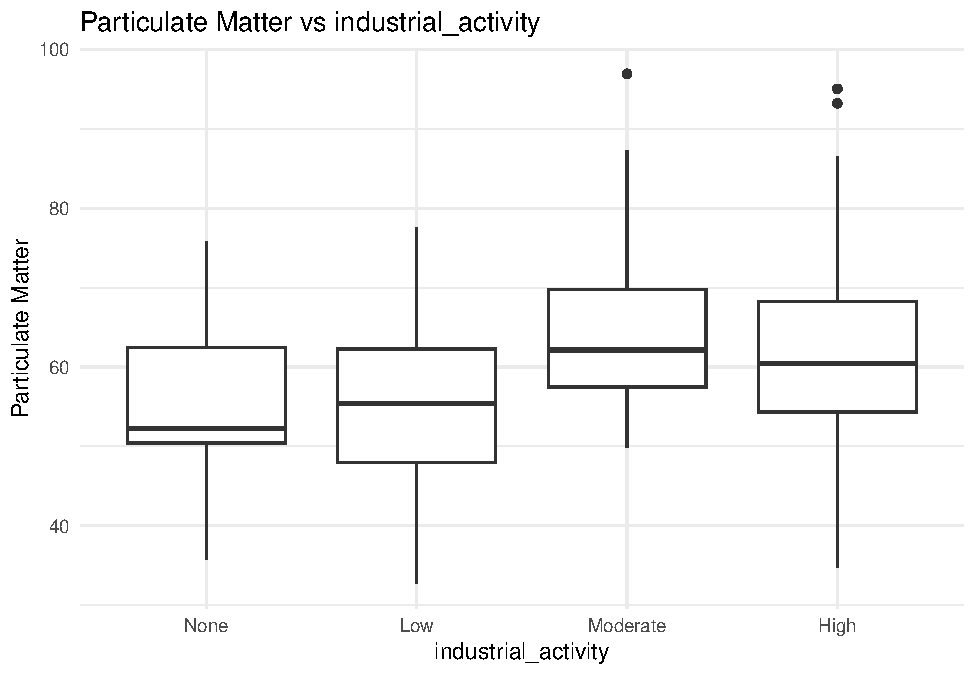
\includegraphics{Report_files/figure-latex/unnamed-chunk-2-1.pdf}
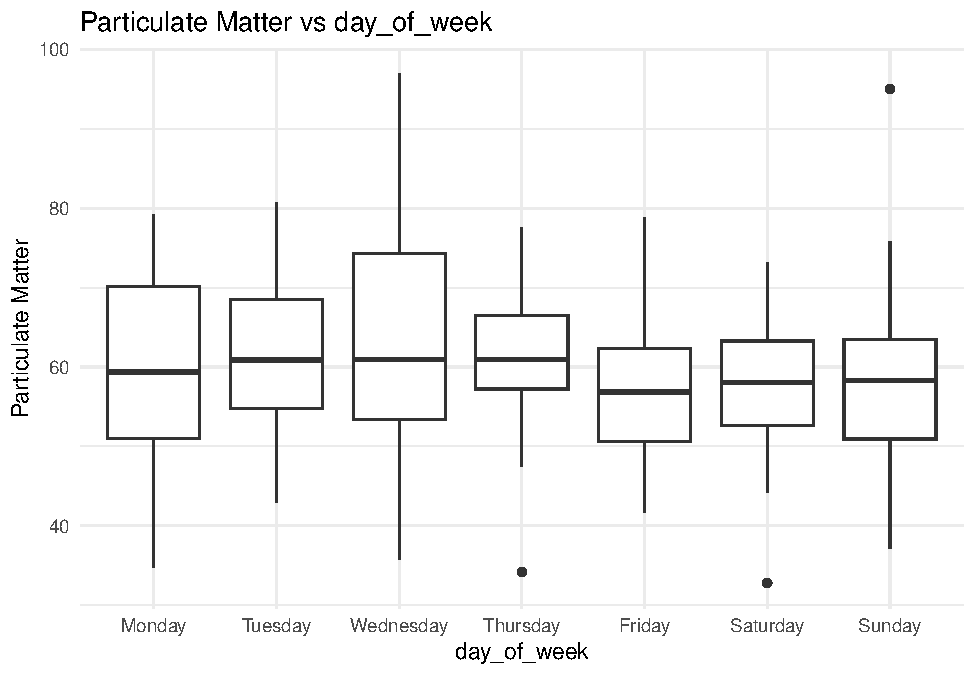
\includegraphics{Report_files/figure-latex/unnamed-chunk-2-2.pdf}
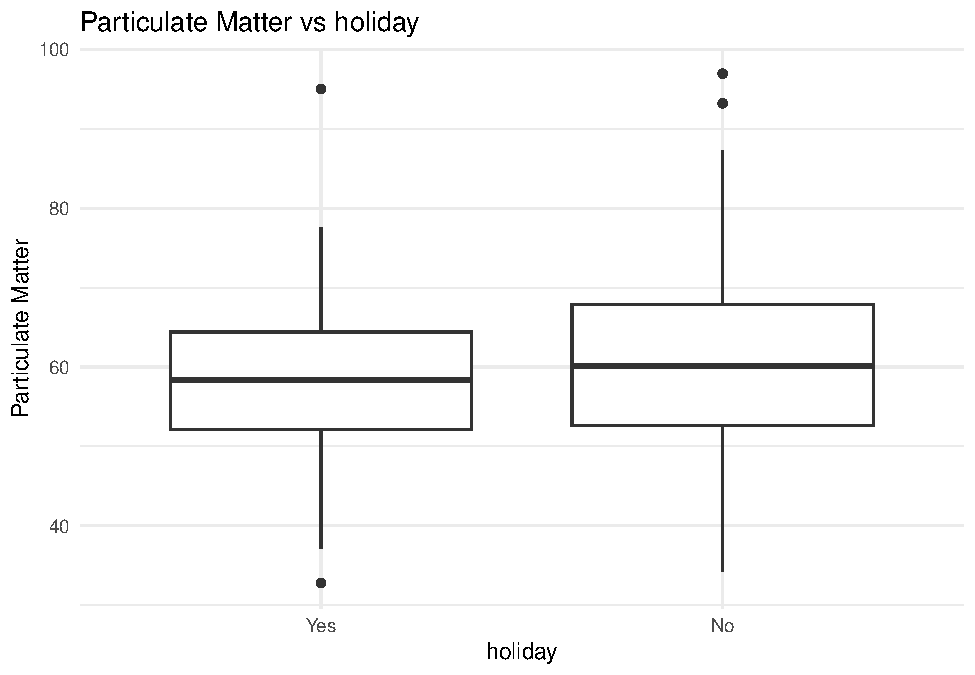
\includegraphics{Report_files/figure-latex/unnamed-chunk-2-3.pdf}
tabular representation of relationship between categorial variables

\begin{Shaded}
\begin{Highlighting}[]
\ControlFlowTok{for}\NormalTok{ (i }\ControlFlowTok{in} \DecValTok{1}\SpecialCharTok{:}\NormalTok{(}\FunctionTok{length}\NormalTok{(categorical\_vars)}\SpecialCharTok{{-}}\DecValTok{1}\NormalTok{)) \{}
  \ControlFlowTok{for}\NormalTok{ (j }\ControlFlowTok{in}\NormalTok{ (i}\SpecialCharTok{+}\DecValTok{1}\NormalTok{)}\SpecialCharTok{:}\FunctionTok{length}\NormalTok{(categorical\_vars)) \{}
    \FunctionTok{cat}\NormalTok{(}\StringTok{"Contingency Table for"}\NormalTok{, categorical\_vars[i], }\StringTok{"and"}\NormalTok{, categorical\_vars[j], }\StringTok{"}\SpecialCharTok{\textbackslash{}n}\StringTok{"}\NormalTok{)}
    \FunctionTok{print}\NormalTok{(}\FunctionTok{table}\NormalTok{(data\_tidy\_air\_quality[[categorical\_vars[i]]], data\_tidy\_air\_quality[[categorical\_vars[j]]]))}
    \FunctionTok{cat}\NormalTok{(}\StringTok{"}\SpecialCharTok{\textbackslash{}n}\StringTok{"}\NormalTok{)}
\NormalTok{  \}}
\NormalTok{\}}
\end{Highlighting}
\end{Shaded}

\begin{verbatim}
## Contingency Table for industrial_activity and day_of_week 
##           
##            Monday Tuesday Wednesday Thursday Friday Saturday Sunday
##   None          2       0         3        3      2        0      4
##   Low           5       6         4        7      6        9      4
##   Moderate      4       4        10        8      6        4      3
##   High         11       7         9        5      8       10      6
## 
## Contingency Table for industrial_activity and holiday 
##           
##            Yes No
##   None       5  9
##   Low       17 24
##   Moderate   9 30
##   High      21 35
## 
## Contingency Table for day_of_week and holiday 
##            
##             Yes No
##   Monday      1 21
##   Tuesday     1 16
##   Wednesday   3 23
##   Thursday    4 19
##   Friday      3 19
##   Saturday   23  0
##   Sunday     17  0
\end{verbatim}

visual representation of relationship between categorial variables

\begin{Shaded}
\begin{Highlighting}[]
\ControlFlowTok{for}\NormalTok{ (i }\ControlFlowTok{in} \DecValTok{1}\SpecialCharTok{:}\NormalTok{(}\FunctionTok{length}\NormalTok{(categorical\_vars) }\SpecialCharTok{{-}} \DecValTok{1}\NormalTok{)) \{}
  \ControlFlowTok{for}\NormalTok{ (j }\ControlFlowTok{in}\NormalTok{ (i }\SpecialCharTok{+} \DecValTok{1}\NormalTok{)}\SpecialCharTok{:}\FunctionTok{length}\NormalTok{(categorical\_vars)) \{}
    \CommentTok{\# Create the plot}
\NormalTok{    p }\OtherTok{\textless{}{-}} \FunctionTok{ggplot}\NormalTok{(data\_tidy\_air\_quality, }\FunctionTok{aes\_string}\NormalTok{(}\AttributeTok{x =}\NormalTok{ categorical\_vars[i], }\AttributeTok{fill =}\NormalTok{ categorical\_vars[j])) }\SpecialCharTok{+}
      \FunctionTok{geom\_bar}\NormalTok{(}\AttributeTok{position =} \StringTok{"fill"}\NormalTok{) }\SpecialCharTok{+}  \CommentTok{\# Use "fill" to make it a stacked bar chart (proportions)}
      \FunctionTok{labs}\NormalTok{(}\AttributeTok{title =} \FunctionTok{paste}\NormalTok{(}\StringTok{"Stacked Bar Chart of"}\NormalTok{, categorical\_vars[i], }\StringTok{"and"}\NormalTok{, categorical\_vars[j]),}
           \AttributeTok{x =}\NormalTok{ categorical\_vars[i],}
           \AttributeTok{y =} \StringTok{"Proportion"}\NormalTok{) }\SpecialCharTok{+}
      \FunctionTok{theme\_minimal}\NormalTok{() }\SpecialCharTok{+}
      \FunctionTok{theme}\NormalTok{(}\AttributeTok{axis.text.x =} \FunctionTok{element\_text}\NormalTok{(}\AttributeTok{angle =} \DecValTok{45}\NormalTok{, }\AttributeTok{hjust =} \DecValTok{1}\NormalTok{))}
    
    \CommentTok{\# Print the plot}
    \FunctionTok{print}\NormalTok{(p)}
\NormalTok{  \}}
\NormalTok{\}}
\end{Highlighting}
\end{Shaded}

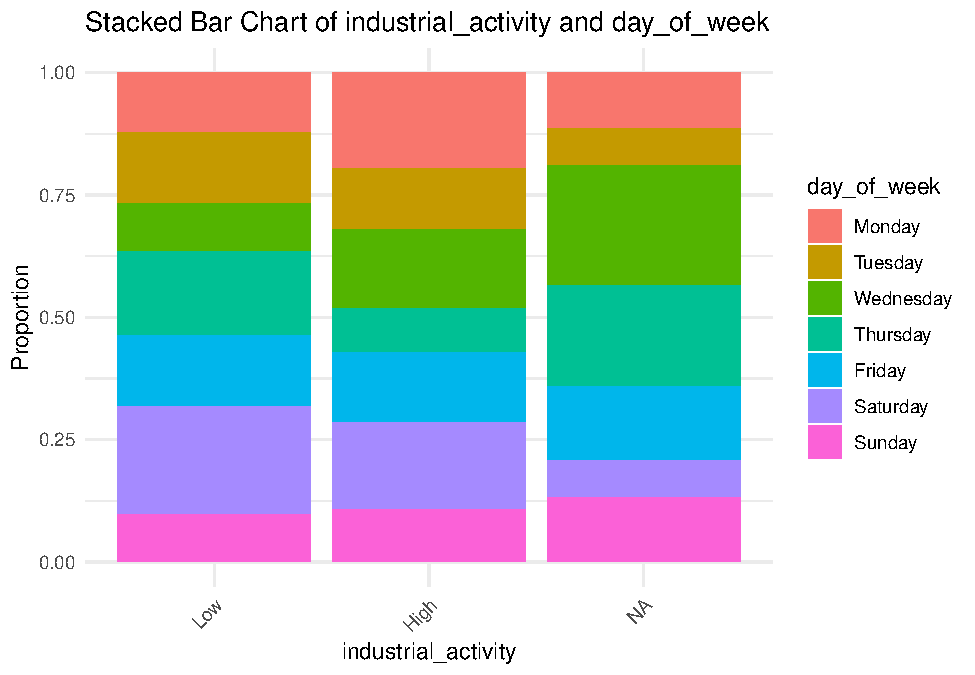
\includegraphics{Report_files/figure-latex/unnamed-chunk-4-1.pdf}
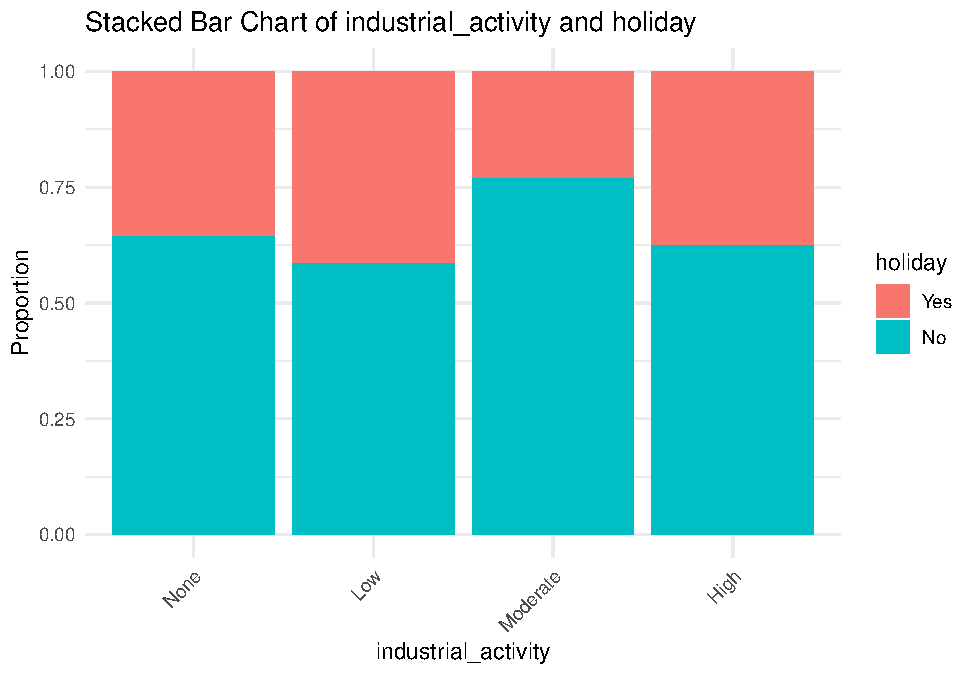
\includegraphics{Report_files/figure-latex/unnamed-chunk-4-2.pdf}
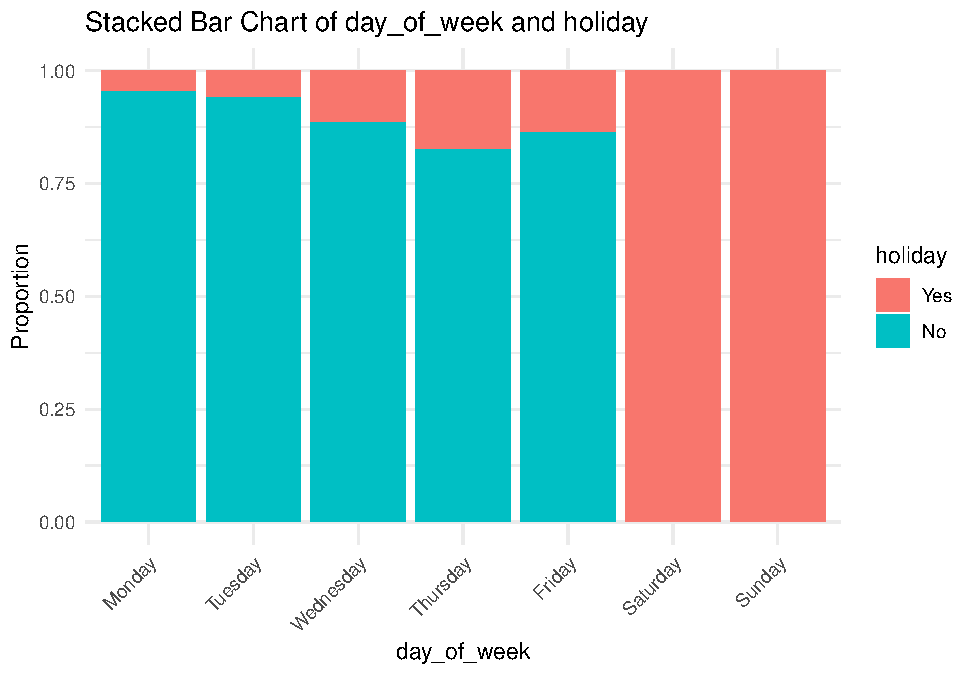
\includegraphics{Report_files/figure-latex/unnamed-chunk-4-3.pdf}
comments\\
distribution characterisitcs\\
The distribution of particulate matter levels is generally right-skewed,
indicating that a small number of observations have significantly high
levels of particulate matter while most observations are clustered at
lower levels. The presence of outliers suggests variations in local
conditions affecting air quality.\\
Observed Relationships\\
1. Traffic Density: A positive correlation exists between particulate
matter levels and traffic density, suggesting that areas with higher
vehicle traffic tend to experience elevated levels of particulate
matter.\\
2. Urban Greenery: A negative trend is observed, where higher urban
greenery correlates with lower particulate matter, indicating that
vegetation may help mitigate air pollution.\\
3. Temperature and Wind Speed: No strong relationship was identified
between particulate matter and temperature. However, there is a slight
negative correlation with wind speed, indicating that higher wind speeds
may help disperse particulate matter.

Potential Collinearity\\
Some potential collinearity is observed among the explanatory variables,
particularly between traffic density and urban greenery. High traffic
areas often have less vegetation, leading to a relationship that may
confound the analysis. Additionally, temperature and wind speed may also
exhibit collinearity, as changes in one could affect the other.

\hypertarget{section-3}{%
\section{Section 3}\label{section-3}}

simple linear regression

\begin{Shaded}
\begin{Highlighting}[]
\NormalTok{X }\OtherTok{\textless{}{-}} \FunctionTok{cbind}\NormalTok{(}\DecValTok{1}\NormalTok{,data\_tidy\_air\_quality}\SpecialCharTok{$}\NormalTok{traffic\_density)}

\NormalTok{Y }\OtherTok{\textless{}{-}}\NormalTok{data\_tidy\_air\_quality}\SpecialCharTok{$}\NormalTok{particulate\_matter}
\NormalTok{bhat }\OtherTok{\textless{}{-}} \FunctionTok{solve}\NormalTok{(}\FunctionTok{t}\NormalTok{(X) }\SpecialCharTok{\%*\%}\NormalTok{ X) }\SpecialCharTok{\%*\%} \FunctionTok{t}\NormalTok{(X) }\SpecialCharTok{\%*\%}\NormalTok{ Y}

\NormalTok{Cmat }\OtherTok{\textless{}{-}} \FunctionTok{solve}\NormalTok{(}\FunctionTok{t}\NormalTok{(X) }\SpecialCharTok{\%*\%}\NormalTok{ X)}

\NormalTok{k }\OtherTok{\textless{}{-}} \FunctionTok{ncol}\NormalTok{(X)}
\NormalTok{rss }\OtherTok{\textless{}{-}} \FunctionTok{t}\NormalTok{(Y }\SpecialCharTok{{-}}\NormalTok{ X }\SpecialCharTok{\%*\%}\NormalTok{ bhat) }\SpecialCharTok{\%*\%}\NormalTok{ (Y }\SpecialCharTok{{-}}\NormalTok{ X }\SpecialCharTok{\%*\%}\NormalTok{ bhat)}
\CommentTok{\# Calculate s2 = RSS/(n{-}k)}
\NormalTok{s2 }\OtherTok{\textless{}{-}} \FunctionTok{as.numeric}\NormalTok{((rss)}\SpecialCharTok{/}\DecValTok{148}\NormalTok{)}
\NormalTok{s2}
\end{Highlighting}
\end{Shaded}

\begin{verbatim}
## [1] 143.5745
\end{verbatim}

\begin{Shaded}
\begin{Highlighting}[]
\NormalTok{c\_ii }\OtherTok{\textless{}{-}} \FunctionTok{diag}\NormalTok{(Cmat)}

\NormalTok{std.error }\OtherTok{\textless{}{-}} \FunctionTok{sqrt}\NormalTok{(s2 }\SpecialCharTok{*}\NormalTok{ c\_ii)}
\NormalTok{std.error}
\end{Highlighting}
\end{Shaded}

\begin{verbatim}
## [1] 20.37801682  0.04065266
\end{verbatim}

\begin{Shaded}
\begin{Highlighting}[]
\NormalTok{mod1}\OtherTok{\textless{}{-}}\FunctionTok{lm}\NormalTok{(data\_tidy\_air\_quality}\SpecialCharTok{$}\NormalTok{particulate\_matter }\SpecialCharTok{\textasciitilde{}}\NormalTok{ data\_tidy\_air\_quality}\SpecialCharTok{$}\NormalTok{traffic\_density, }\AttributeTok{data =}\NormalTok{ data\_tidy\_air\_quality)}

\FunctionTok{summary}\NormalTok{(mod1)}
\end{Highlighting}
\end{Shaded}

\begin{verbatim}
## 
## Call:
## lm(formula = data_tidy_air_quality$particulate_matter ~ data_tidy_air_quality$traffic_density, 
##     data = data_tidy_air_quality)
## 
## Residuals:
##     Min      1Q  Median      3Q     Max 
## -28.332  -7.561  -1.050   6.110  35.243 
## 
## Coefficients:
##                                       Estimate Std. Error t value Pr(>|t|)  
## (Intercept)                           18.11537   20.37802   0.889   0.3755  
## data_tidy_air_quality$traffic_density  0.08400    0.04065   2.066   0.0406 *
## ---
## Signif. codes:  0 '***' 0.001 '**' 0.01 '*' 0.05 '.' 0.1 ' ' 1
## 
## Residual standard error: 11.98 on 148 degrees of freedom
## Multiple R-squared:  0.02804,    Adjusted R-squared:  0.02147 
## F-statistic: 4.269 on 1 and 148 DF,  p-value: 0.04055
\end{verbatim}

hypthesis test

\begin{Shaded}
\begin{Highlighting}[]
\CommentTok{\# Summary of ANOVA results}
\FunctionTok{summary}\NormalTok{(}\FunctionTok{aov}\NormalTok{(particulate\_matter }\SpecialCharTok{\textasciitilde{}}\NormalTok{ industrial\_activity, }\AttributeTok{data =}\NormalTok{ data\_tidy\_air\_quality))}
\end{Highlighting}
\end{Shaded}

\begin{verbatim}
##                      Df Sum Sq Mean Sq F value Pr(>F)   
## industrial_activity   3   2182   727.3   5.396 0.0015 **
## Residuals           146  19680   134.8                  
## ---
## Signif. codes:  0 '***' 0.001 '**' 0.01 '*' 0.05 '.' 0.1 ' ' 1
\end{verbatim}

\begin{Shaded}
\begin{Highlighting}[]
\CommentTok{\# Calculate F{-}statistic and p{-}value manually}
\NormalTok{group\_means }\OtherTok{\textless{}{-}} \FunctionTok{tapply}\NormalTok{(data\_tidy\_air\_quality}\SpecialCharTok{$}\NormalTok{particulate\_matter, data\_tidy\_air\_quality}\SpecialCharTok{$}\NormalTok{industrial\_activity, mean)}
\NormalTok{overall\_mean }\OtherTok{\textless{}{-}} \FunctionTok{mean}\NormalTok{(data\_tidy\_air\_quality}\SpecialCharTok{$}\NormalTok{particulate\_matter)}

\CommentTok{\# Calculate SST}
\NormalTok{SST }\OtherTok{\textless{}{-}} \FunctionTok{sum}\NormalTok{((data\_tidy\_air\_quality}\SpecialCharTok{$}\NormalTok{particulate\_matter }\SpecialCharTok{{-}}\NormalTok{ overall\_mean)}\SpecialCharTok{\^{}}\DecValTok{2}\NormalTok{)}

\CommentTok{\# Calculate SSB}
\NormalTok{n }\OtherTok{\textless{}{-}} \FunctionTok{table}\NormalTok{(data\_tidy\_air\_quality}\SpecialCharTok{$}\NormalTok{industrial\_activity)}
\NormalTok{SStreatment }\OtherTok{\textless{}{-}} \FunctionTok{sum}\NormalTok{(n }\SpecialCharTok{*}\NormalTok{ (group\_means }\SpecialCharTok{{-}}\NormalTok{ overall\_mean)}\SpecialCharTok{\^{}}\DecValTok{2}\NormalTok{)}

\CommentTok{\# Calculate SSW}
\NormalTok{group\_means\_vector }\OtherTok{\textless{}{-}} \FunctionTok{unlist}\NormalTok{(}\FunctionTok{tapply}\NormalTok{(data\_tidy\_air\_quality}\SpecialCharTok{$}\NormalTok{particulate\_matter, data\_tidy\_air\_quality}\SpecialCharTok{$}\NormalTok{industrial\_activity, mean)[data\_tidy\_air\_quality}\SpecialCharTok{$}\NormalTok{industrial\_activity])}
\NormalTok{SSerror }\OtherTok{\textless{}{-}} \FunctionTok{sum}\NormalTok{((data\_tidy\_air\_quality}\SpecialCharTok{$}\NormalTok{particulate\_matter }\SpecialCharTok{{-}}\NormalTok{ group\_means\_vector)}\SpecialCharTok{\^{}}\DecValTok{2}\NormalTok{)}

\CommentTok{\# Calculate degrees of freedom}
\NormalTok{k }\OtherTok{\textless{}{-}} \FunctionTok{length}\NormalTok{(}\FunctionTok{unique}\NormalTok{(data\_tidy\_air\_quality}\SpecialCharTok{$}\NormalTok{industrial\_activity))}
\NormalTok{N }\OtherTok{\textless{}{-}} \FunctionTok{nrow}\NormalTok{(data)}
\NormalTok{DFtreatment }\OtherTok{\textless{}{-}}\NormalTok{ k }\SpecialCharTok{{-}} \DecValTok{1}
\NormalTok{DFerror }\OtherTok{\textless{}{-}} \DecValTok{150} \SpecialCharTok{{-}}\NormalTok{ k}

\CommentTok{\# Calculate Mean Squares}
\NormalTok{MStreatment }\OtherTok{\textless{}{-}}\NormalTok{ SStreatment }\SpecialCharTok{/}\NormalTok{ DFtreatment}
\NormalTok{MSerror }\OtherTok{\textless{}{-}}\NormalTok{ SSerror }\SpecialCharTok{/}\NormalTok{ DFerror}


\CommentTok{\# Calculate F{-}statistic}
\NormalTok{F\_statistic }\OtherTok{\textless{}{-}}\NormalTok{ MStreatment}\SpecialCharTok{/}\NormalTok{MSerror}

\CommentTok{\# Output F{-}statistic}
\NormalTok{F\_statistic}
\end{Highlighting}
\end{Shaded}

\begin{verbatim}
## [1] 5.395959
\end{verbatim}

\begin{Shaded}
\begin{Highlighting}[]
\CommentTok{\# Calculate p{-}value}
\NormalTok{p\_value }\OtherTok{\textless{}{-}} \FunctionTok{pf}\NormalTok{(F\_statistic, DFtreatment, DFerror, }\AttributeTok{lower.tail =} \ConstantTok{FALSE}\NormalTok{)}
\NormalTok{p\_value}
\end{Highlighting}
\end{Shaded}

\begin{verbatim}
## [1] 0.001502236
\end{verbatim}

\newpage

\hypertarget{question-4}{%
\section{Question 4}\label{question-4}}

\begingroup\fontsize{12}{14}\selectfont

\begin{longtable}[t]{lccc}
\caption{\label{tab:unnamed-chunk-7}Confidence Interval for each Coefficients}\\
\toprule
 & 2.5 \% & Estimate & 97.5 \%\\
\midrule
\addlinespace[0.3em]
\multicolumn{4}{l}{\textbf{Intercept}}\\
\hspace{1em}(Intercept) & -21.0568 & 13.7937 & 48.6442\\
\addlinespace[0.3em]
\multicolumn{4}{l}{\textbf{Traffic Density}}\\
\hspace{1em}traffic\_density & 0.0155 & 0.0799 & 0.1444\\
\addlinespace[0.3em]
\multicolumn{4}{l}{\textbf{Industrial Activity}}\\
\hspace{1em}industrial\_activityLow & -3.1721 & 2.6589 & 8.4900\\
\hspace{1em}industrial\_activityModerate & 0.6047 & 6.4545 & 12.3043\\
\hspace{1em}industrial\_activityHigh & -0.2503 & 5.3652 & 10.9806\\
\addlinespace[0.3em]
\multicolumn{4}{l}{\textbf{Natural Factors}}\\
\hspace{1em}temperature & -1.1521 & -0.2815 & 0.5891\\
\hspace{1em}humidity & -0.1111 & 0.1926 & 0.4962\\
\hspace{1em}wind\_speed & -0.8040 & 0.0193 & 0.8426\\
\hspace{1em}temperature:humidity & -0.0088 & 0.0061 & 0.0209\\
\addlinespace[0.3em]
\multicolumn{4}{l}{\textbf{Day of Week}}\\
\hspace{1em}day\_of\_weekTuesday & -5.9877 & 0.0133 & 6.0142\\
\hspace{1em}day\_of\_weekWednesday & -5.3501 & 0.1565 & 5.6630\\
\hspace{1em}day\_of\_weekThursday & -5.5367 & 0.1662 & 5.8690\\
\hspace{1em}day\_of\_weekFriday & -8.0602 & -2.4221 & 3.2161\\
\hspace{1em}day\_of\_weekSaturday & -12.3605 & -4.4832 & 3.3940\\
\hspace{1em}day\_of\_weekSunday & -10.2167 & -2.0885 & 6.0396\\
\addlinespace[0.3em]
\multicolumn{4}{l}{\textbf{Holiday}}\\
\hspace{1em}holidayNo & -6.7151 & -0.9961 & 4.7228\\
\addlinespace[0.3em]
\multicolumn{4}{l}{\textbf{Urban Greenery}}\\
\hspace{1em}urban\_greenery & -0.4142 & -0.2954 & -0.1766\\
\bottomrule
\end{longtable}
\endgroup{}

\hypertarget{hypothesis-testing}{%
\subsubsection{Hypothesis Testing}\label{hypothesis-testing}}

We'd like to perform hypothesis tests on the following variables:
Temperature, Humidity, Industrial Levels, and Day of Week.

We'll start by examining whether Temperature has an effect on the
concentration of Particulate Matter. We'll use the following We use the
following set of hypothesis:

\begin{Shaded}
\begin{Highlighting}[]
\CommentTok{\#\textbackslash{}begin\{align\}}
\CommentTok{\#$$H\_0: \textbackslash{}beta\_\{temp\} = \textbackslash{}beta\_\{hum:temp\} = 0$$ }
\CommentTok{\#$$H\_A: \textbackslash{}beta\_\{temp\} \textbackslash{}neq 0 \textbackslash{}text\{ and \} \textbackslash{}beta\_\{hum:temp\} \textbackslash{}neq 0$$}
\CommentTok{\#\textbackslash{}end\{align\}}
\CommentTok{\#\textbackslash{}}
\CommentTok{\#This can be done by comparing the restricted and un restricted model:}
\CommentTok{\#$$Y\_R = \textbackslash{}beta\_0 + \textbackslash{}beta\_\{traffic\}X + $$}
\end{Highlighting}
\end{Shaded}

\begin{Shaded}
\begin{Highlighting}[]
\NormalTok{model\_unrestricted }\OtherTok{\textless{}{-}} \FunctionTok{lm}\NormalTok{(particulate\_matter }\SpecialCharTok{\textasciitilde{}}\NormalTok{ . }\SpecialCharTok{+} 
\NormalTok{                         temperature}\SpecialCharTok{:}\NormalTok{humidity,}
                         \AttributeTok{data=}\NormalTok{data\_tidy\_air\_quality)}
\NormalTok{model\_restricted }\OtherTok{\textless{}{-}} \FunctionTok{update}\NormalTok{(model\_unrestricted, .}\SpecialCharTok{\textasciitilde{}}\NormalTok{.}
                           \SpecialCharTok{{-}}\NormalTok{ temperature}
                           \SpecialCharTok{{-}}\NormalTok{ temperature}\SpecialCharTok{:}\NormalTok{humidity)}
\FunctionTok{anova}\NormalTok{(model\_unrestricted, model\_restricted)}
\end{Highlighting}
\end{Shaded}

\begin{verbatim}
## Analysis of Variance Table
## 
## Model 1: particulate_matter ~ traffic_density + industrial_activity + 
##     temperature + humidity + wind_speed + day_of_week + holiday + 
##     urban_greenery + temperature:humidity
## Model 2: particulate_matter ~ traffic_density + industrial_activity + 
##     humidity + wind_speed + day_of_week + holiday + urban_greenery
##   Res.Df   RSS Df Sum of Sq      F Pr(>F)
## 1    133 11032                           
## 2    135 11096 -2   -63.801 0.3846 0.6815
\end{verbatim}

Using the anova function in R, we compare the two models with F test,
yielding a P value 0.6815, suggesting that temperature doesn't have a
significant effect on the concentration of particular matter.

\hypertarget{part-2}{%
\section{part 2}\label{part-2}}

scenario A

\begin{Shaded}
\begin{Highlighting}[]
\FunctionTok{library}\NormalTok{(tidyverse)}
\end{Highlighting}
\end{Shaded}

\begin{verbatim}
## Warning: package 'tidyverse' was built under R version 4.3.3
\end{verbatim}

\begin{verbatim}
## Warning: package 'lubridate' was built under R version 4.3.3
\end{verbatim}

\begin{verbatim}
## -- Attaching core tidyverse packages ------------------------ tidyverse 2.0.0 --
## v dplyr     1.1.2     v readr     2.1.4
## v forcats   1.0.0     v stringr   1.5.0
## v lubridate 1.9.3     v tibble    3.2.1
## v purrr     1.0.2     
## -- Conflicts ------------------------------------------ tidyverse_conflicts() --
## x dplyr::filter()     masks stats::filter()
## x dplyr::group_rows() masks kableExtra::group_rows()
## x dplyr::lag()        masks stats::lag()
## i Use the conflicted package (<http://conflicted.r-lib.org/>) to force all conflicts to become errors
\end{verbatim}

\begin{Shaded}
\begin{Highlighting}[]
\CommentTok{\# Set the seed for reproducibility}
\FunctionTok{set.seed}\NormalTok{(}\DecValTok{123}\NormalTok{)}

\CommentTok{\# Number of simulations}
\NormalTok{n\_simulations }\OtherTok{\textless{}{-}} \DecValTok{1000}

\NormalTok{temperature }\OtherTok{\textless{}{-}}\NormalTok{ data\_tidy\_air\_quality}\SpecialCharTok{$}\NormalTok{temperature}

\CommentTok{\# Initialize a vector to store whether the null hypothesis was rejected in each simulation}
\NormalTok{reject\_null }\OtherTok{\textless{}{-}} \FunctionTok{numeric}\NormalTok{(n\_simulations)}


\CommentTok{\# Variance of the uniform distribution needs to be 100, so we calculated b = 17.32}
\NormalTok{a }\OtherTok{\textless{}{-}} \SpecialCharTok{{-}}\FloatTok{17.32}
\NormalTok{b }\OtherTok{\textless{}{-}} \FloatTok{17.32}

\CommentTok{\# Run simulations}
\ControlFlowTok{for}\NormalTok{ (i }\ControlFlowTok{in} \DecValTok{1}\SpecialCharTok{:}\NormalTok{n\_simulations) \{}
  
  \CommentTok{\# Generate error term e \textasciitilde{} Uniform(a, b)}
\NormalTok{  e }\OtherTok{\textless{}{-}} \FunctionTok{runif}\NormalTok{(}\FunctionTok{length}\NormalTok{(temperature), }\AttributeTok{min =}\NormalTok{ a, }\AttributeTok{max =}\NormalTok{ b)}
  
  \CommentTok{\# Generate Y = 30 + e (since β1 = 0)}
\NormalTok{  Y }\OtherTok{\textless{}{-}} \DecValTok{30} \SpecialCharTok{+}\NormalTok{ e}
  
  
  \CommentTok{\# Fit the linear model Y = β0 + β1 * temperature}
\NormalTok{  model }\OtherTok{\textless{}{-}} \FunctionTok{lm}\NormalTok{(Y }\SpecialCharTok{\textasciitilde{}}\NormalTok{ temperature)}
  
  \CommentTok{\# Perform hypothesis test on β1 (null hypothesis: β1 = 0) and extract from lm}
\NormalTok{  p\_value }\OtherTok{\textless{}{-}} \FunctionTok{summary}\NormalTok{(model)}\SpecialCharTok{$}\NormalTok{coefficients[}\DecValTok{2}\NormalTok{, }\DecValTok{4}\NormalTok{]}
\NormalTok{  p\_value}
  
  \CommentTok{\# Record if the null hypothesis is rejected (α = 0.05)}
\NormalTok{  reject\_null[i] }\OtherTok{\textless{}{-}} \FunctionTok{ifelse}\NormalTok{(p\_value }\SpecialCharTok{\textless{}} \FloatTok{0.05}\NormalTok{, }\DecValTok{1}\NormalTok{, }\DecValTok{0}\NormalTok{)}

\NormalTok{  \}}

\CommentTok{\# Calculate Type I error rate (proportion of times the null was incorrectly rejected)}
\NormalTok{type\_1\_error\_rate }\OtherTok{\textless{}{-}}\NormalTok{(}\DecValTok{1000}\SpecialCharTok{{-}}\FunctionTok{sum}\NormalTok{(reject\_null))}\SpecialCharTok{/}\DecValTok{1000}

\CommentTok{\# Output the Type I error rate}

\NormalTok{type\_1\_error\_rate}
\end{Highlighting}
\end{Shaded}

\begin{verbatim}
## [1] 0.957
\end{verbatim}

Methodology for Scenario A: Simulation under the null hypothesis
(\(\beta_{1}\) = 0): We simulate the model assuming there is no effect
of temperature on particulate matter (i.e., \(\beta_{1}\) = 0). Hence,
the model simplifies to: \begin{align}
$$Y_{i}= 30 + e_{i} $$
\end{align}

scenario b

\begin{Shaded}
\begin{Highlighting}[]
\FunctionTok{set.seed}\NormalTok{(}\DecValTok{123}\NormalTok{)  }\CommentTok{\# For reproducibility}

\CommentTok{\# Load data (assuming temperature values are stored in \textquotesingle{}temperature\textquotesingle{} variable)}
\NormalTok{temperature }\OtherTok{\textless{}{-}}\NormalTok{ data\_tidy\_air\_quality}\SpecialCharTok{$}\NormalTok{temperature}

\NormalTok{n }\OtherTok{\textless{}{-}} \FunctionTok{length}\NormalTok{(temperature)  }\CommentTok{\# Number of observations in temperature data}


\NormalTok{reject\_null }\OtherTok{\textless{}{-}} \FunctionTok{numeric}\NormalTok{(n\_simulations)  }\CommentTok{\# To store whether the null hypothesis is rejected}

\ControlFlowTok{for}\NormalTok{ (i }\ControlFlowTok{in} \DecValTok{1}\SpecialCharTok{:}\NormalTok{n\_simulations) \{}
  \CommentTok{\# Simulate heteroscedastic errors with mean variance 100 and variance of the variances = 50}
  \CommentTok{\# Generate different variances for each observation, ensuring mean is 100 and variance is 50}
\NormalTok{  variances }\OtherTok{\textless{}{-}} \FunctionTok{rnorm}\NormalTok{(n, }\AttributeTok{mean =} \DecValTok{100}\NormalTok{, }\AttributeTok{sd =} \FunctionTok{sqrt}\NormalTok{(}\DecValTok{50}\NormalTok{))  }\CommentTok{\# Variance of each error term}
\NormalTok{  e }\OtherTok{\textless{}{-}} \FunctionTok{rnorm}\NormalTok{(n, }\AttributeTok{mean =} \DecValTok{0}\NormalTok{, }\AttributeTok{sd =} \FunctionTok{sqrt}\NormalTok{(}\FunctionTok{abs}\NormalTok{(variances)))  }\CommentTok{\# Simulated errors with heteroscedasticity}
  
  \CommentTok{\# Generate Y values under null hypothesis (beta\_1 = 0)}
\NormalTok{  Y }\OtherTok{\textless{}{-}} \DecValTok{30} \SpecialCharTok{+}\NormalTok{ e}
  
  \CommentTok{\# Fit the model Y \textasciitilde{} temperature}
\NormalTok{  model }\OtherTok{\textless{}{-}} \FunctionTok{lm}\NormalTok{(Y }\SpecialCharTok{\textasciitilde{}}\NormalTok{ temperature)}
  
  \CommentTok{\# Perform hypothesis test for beta\_1 (test if beta\_1 = 0)}
\NormalTok{  p\_value }\OtherTok{\textless{}{-}} \FunctionTok{summary}\NormalTok{(model)}\SpecialCharTok{$}\NormalTok{coefficients[}\DecValTok{2}\NormalTok{, }\DecValTok{4}\NormalTok{]  }\CommentTok{\# Extract p{-}value for temperature coefficient}
  
  \CommentTok{\# Record whether the null hypothesis is rejected (p{-}value \textless{} 0.05)}
\NormalTok{  reject\_null[i] }\OtherTok{\textless{}{-}} \FunctionTok{as.numeric}\NormalTok{(p\_value }\SpecialCharTok{\textless{}} \FloatTok{0.05}\NormalTok{)}
\NormalTok{\}}

\CommentTok{\# Calculate the Type I error rate (proportion of rejected null hypotheses)}
\NormalTok{type\_1\_error\_rate }\OtherTok{\textless{}{-}}\NormalTok{ (}\DecValTok{1000}\SpecialCharTok{{-}}\FunctionTok{sum}\NormalTok{(reject\_null))}\SpecialCharTok{/}\DecValTok{1000}

\CommentTok{\# Print the Type I error rate}
\NormalTok{type\_1\_error\_rate}
\end{Highlighting}
\end{Shaded}

\begin{verbatim}
## [1] 0.953
\end{verbatim}

scenario C

\begin{Shaded}
\begin{Highlighting}[]
\FunctionTok{set.seed}\NormalTok{(}\DecValTok{123}\NormalTok{)  }\CommentTok{\# For reproducibility}

\CommentTok{\# Load data (assuming temperature values are stored in \textquotesingle{}temperature\textquotesingle{} variable)}
\NormalTok{temperature }\OtherTok{\textless{}{-}}\NormalTok{ data\_tidy\_air\_quality}\SpecialCharTok{$}\NormalTok{temperature}

\NormalTok{n }\OtherTok{\textless{}{-}} \FunctionTok{length}\NormalTok{(temperature)  }\CommentTok{\# Number of observations in temperature data}
\NormalTok{n\_sim }\OtherTok{\textless{}{-}} \DecValTok{1000}  \CommentTok{\# Number of simulations}

\CommentTok{\# Function to generate autocorrelated errors}
\NormalTok{generate\_ar1\_errors }\OtherTok{\textless{}{-}} \ControlFlowTok{function}\NormalTok{(n, rho, var\_epsilon) \{}
\NormalTok{  sigma\_u\_squared }\OtherTok{\textless{}{-}}\NormalTok{ var\_epsilon }\SpecialCharTok{*}\NormalTok{ (}\DecValTok{1} \SpecialCharTok{{-}}\NormalTok{ rho}\SpecialCharTok{\^{}}\DecValTok{2}\NormalTok{)}
\NormalTok{  u }\OtherTok{\textless{}{-}} \FunctionTok{rnorm}\NormalTok{(n, }\AttributeTok{mean =} \DecValTok{0}\NormalTok{, }\AttributeTok{sd =} \FunctionTok{sqrt}\NormalTok{(sigma\_u\_squared))}
\NormalTok{  epsilon }\OtherTok{\textless{}{-}} \FunctionTok{numeric}\NormalTok{(n)}
\NormalTok{  epsilon[}\DecValTok{1}\NormalTok{] }\OtherTok{\textless{}{-}}\NormalTok{ u[}\DecValTok{1}\NormalTok{]}
  \ControlFlowTok{for}\NormalTok{ (i }\ControlFlowTok{in} \DecValTok{2}\SpecialCharTok{:}\NormalTok{n) \{}
\NormalTok{    epsilon[i] }\OtherTok{\textless{}{-}}\NormalTok{ rho }\SpecialCharTok{*}\NormalTok{ epsilon[i }\SpecialCharTok{{-}} \DecValTok{1}\NormalTok{] }\SpecialCharTok{+}\NormalTok{ u[i]}
\NormalTok{  \}}
\NormalTok{  epsilon}
\NormalTok{\}}

\NormalTok{rho }\OtherTok{\textless{}{-}} \FloatTok{0.3}  \CommentTok{\# Autocorrelation coefficient}
\NormalTok{var\_epsilon }\OtherTok{\textless{}{-}} \DecValTok{100}  \CommentTok{\# Desired variance of errors}

\NormalTok{reject\_null }\OtherTok{\textless{}{-}} \FunctionTok{numeric}\NormalTok{(n\_sim)  }\CommentTok{\# To store whether the null hypothesis is rejected}

\ControlFlowTok{for}\NormalTok{ (i }\ControlFlowTok{in} \DecValTok{1}\SpecialCharTok{:}\NormalTok{n\_sim) \{}
  \CommentTok{\# Generate autocorrelated errors with Corr(epsilon\_i, epsilon\_(i+1)) = 0.3}
\NormalTok{  e }\OtherTok{\textless{}{-}} \FunctionTok{generate\_ar1\_errors}\NormalTok{(n, rho, var\_epsilon)}
  
  \CommentTok{\# Generate Y values under null hypothesis (beta\_1 = 0)}
\NormalTok{  Y }\OtherTok{\textless{}{-}} \DecValTok{30} \SpecialCharTok{+}\NormalTok{ e}
  
  \CommentTok{\# Fit the model Y \textasciitilde{} temperature}
\NormalTok{  model }\OtherTok{\textless{}{-}} \FunctionTok{lm}\NormalTok{(Y }\SpecialCharTok{\textasciitilde{}}\NormalTok{ temperature)}
  
  \CommentTok{\# Perform hypothesis test for beta\_1 (test if beta\_1 = 0)}
\NormalTok{  p\_value }\OtherTok{\textless{}{-}} \FunctionTok{summary}\NormalTok{(model)}\SpecialCharTok{$}\NormalTok{coefficients[}\DecValTok{2}\NormalTok{, }\DecValTok{4}\NormalTok{]  }\CommentTok{\# Extract p{-}value for temperature coefficient}
  
  \CommentTok{\# Record whether the null hypothesis is rejected (p{-}value \textless{} 0.05)}
\NormalTok{  reject\_null[i] }\OtherTok{\textless{}{-}} \FunctionTok{as.numeric}\NormalTok{(p\_value }\SpecialCharTok{\textless{}} \FloatTok{0.05}\NormalTok{)}
\NormalTok{\}}

\CommentTok{\# Calculate the Type I error rate (proportion of rejected null hypotheses)}
\NormalTok{type\_1\_error\_rate }\OtherTok{\textless{}{-}}\NormalTok{ (}\DecValTok{1000}\SpecialCharTok{{-}}\FunctionTok{sum}\NormalTok{(reject\_null))}\SpecialCharTok{/}\DecValTok{1000}

\CommentTok{\# Print the Type I error rate}
\NormalTok{type\_1\_error\_rate}
\end{Highlighting}
\end{Shaded}

\begin{verbatim}
## [1] 0.947
\end{verbatim}

\end{document}
